%% This template can be used to write a paper for
%% Computer Physics Communications using LaTeX.
%% For authors who want to write a computer program description,
%% an example Program Summary is included that only has to be
%% completed and which will give the correct layout in the
%% preprint and the journal.
%% The `elsarticle' style is used and more information on this style
%% can be found at 
%% http://www.elsevier.com/wps/find/authorsview.authors/elsarticle.
%%
%%
\documentclass[preprint,12pt]{elsarticle}

%% Use the option review to obtain double line spacing
%% \documentclass[preprint,review,12pt]{elsarticle}

%% Use the options 1p,twocolumn; 3p; 3p,twocolumn; 5p; or 5p,twocolumn
%% for a journal layout:
%% \documentclass[final,1p,times]{elsarticle}
%% \documentclass[final,1p,times,twocolumn]{elsarticle}
%% \documentclass[final,3p,times]{elsarticle}
%% \documentclass[final,3p,times,twocolumn]{elsarticle}
%% \documentclass[final,5p,times]{elsarticle}
%% \documentclass[final,5p,times,twocolumn]{elsarticle}

%% if you use PostScript figures in your article
%% use the graphics package for simple commands
%% \usepackage{graphics}
%% or use the graphicx package for more complicated commands
%% \usepackage{graphicx}
%% or use the epsfig package if you prefer to use the old commands
%% \usepackage{epsfig}

%% The amssymb package provides various useful mathematical symbols
\usepackage{amssymb}
%% The amsthm package provides extended theorem environments
%% \usepackage{amsthm}

%% The lineno packages adds line numbers. Start line numbering with
%% \begin{linenumbers}, end it with \end{linenumbers}. Or switch it on
%% for the whole article with \linenumbers after \end{frontmatter}.
%% \usepackage{lineno}

%% natbib.sty is loaded by default. However, natbib options can be
%% provided with \biboptions{...} command. Following options are
%% valid:

%%   round  -  round parentheses are used (default)
%%   square -  square brackets are used   [option]
%%   curly  -  curly braces are used      {option}
%%   angle  -  angle brackets are used    <option>
%%   semicolon  -  multiple citations separated by semi-colon
%%   colon  - same as semicolon, an earlier confusion
%%   comma  -  separated by comma
%%   numbers-  selects numerical citations
%%   super  -  numerical citations as superscripts
%%   sort   -  sorts multiple citations according to order in ref. list
%%   sort&compress   -  like sort, but also compresses numerical citations
%%   compress - compresses without sorting
%%
%% \biboptions{comma,round}

% \biboptions{}

\newcommand{\be}{\begin{equation}}
\newcommand{\ee}{\end{equation}}
\newcommand{\ba}{\begin{eqnarray}}
\newcommand{\ea}{\end{eqnarray}}

%% This list environment is used for the references in the
%% Program Summary
%%
\newcounter{bla}
\newenvironment{refnummer}{%
\list{[\arabic{bla}]}%
{\usecounter{bla}%
 \setlength{\itemindent}{0pt}%
 \setlength{\topsep}{0pt}%
 \setlength{\itemsep}{0pt}%
 \setlength{\labelsep}{2pt}%
 \setlength{\listparindent}{0pt}%
 \settowidth{\labelwidth}{[9]}%
 \setlength{\leftmargin}{\labelwidth}%
 \addtolength{\leftmargin}{\labelsep}%
 \setlength{\rightmargin}{0pt}}}
 {\endlist}

\journal{Computer Physics Communications}

\begin{document}

\begin{frontmatter}

%% Title, authors and addresses

%% use the tnoteref command within \title for footnotes;
%% use the tnotetext command for the associated footnote;
%% use the fnref command within \author or \address for footnotes;
%% use the fntext command for the associated footnote;
%% use the corref command within \author for corresponding author footnotes;
%% use the cortext command for the associated footnote;
%% use the ead command for the email address,
%% and the form \ead[url] for the home page:
%%
%% \title{Title\tnoteref{label1}}
%% \tnotetext[label1]{}
%% \author{Name\corref{cor1}\fnref{label2}}
%% \ead{email address}
%% \ead[url]{home page}
%% \fntext[label2]{}
%% \cortext[cor1]{}
%% \address{Address\fnref{label3}}
%% \fntext[label3]{}

\title{{\tt APFELgrid}: a fast interface to hadronic observables for
  fits of parton densities}

%% use optional labels to link authors explicitly to addresses:
%% \author[label1,label2]{<author name>}
%% \address[label1]{<address>}
%% \address[label2]{<address>}

\author[a]{Valerio Bertone}
\author[b]{Stefano Carrazza}
\author[a]{Nathan P. Hartland\corref{author}}

\cortext[author] {Corresponding author.\\\textit{E-mail address:} nathan.hartland@physics.ox.ac.uk}
\address[a]{Rudolf Peierls Centre for Theoretical Physics,\\ 1 Keble Road, University of Oxford, OX1 3NP, Oxford, UK}
\address[b]{TH Unit, CERN, CH-1211 Geneva 23, Switzerland}

\begin{abstract}
We present a new software package designed to aid the inclusion of hadronic
observables into Parton Distribution Function (PDF) fits. The {\tt APFELgrid} package
converts interpolated weight tables provided by {\tt APPLgrid} files into a more efficient
format for PDF fitting by the pre-computation and combination with PDF and $\alpha_s$ evolution factors provided
by {\tt APFEL}. This combination significantly reduces the number of operations required to perform the calculation
of hadronic observables in PDF fits and simplifies the structure of the calculation into
a readily optimised scalar product. We demonstrate that our technique
can lead to a substantial speed improvement as compared to the
existing interfaces without any reduction in numerical accuracy.

%We present a new method conceived to ease the inclusion of hadronic
%observables into parton distribution function (PDF) fits. Our
%technique relies on the the same principles adopted by the existing
%fast interfaces but implements a set of improvements aimed at
%optimizing the performance in the context of PDF fits where many
%iterations and many predictions for each iteration are usually
%required. The main novelties are the precomputation of the PDF and
%$\alpha_s$ evolution and the optimisation of the numerical convolution
%between hard cross sections and PDFs. We demonstrate that our technique
%can lead to a substantial speed improvement as compared to the
%existing interfaces.
\end{abstract}

\begin{keyword}
%% keywords here, in the form: keyword \sep keyword
QCD; parton distribution functions; fast predictions.

\end{keyword}

\end{frontmatter}

\begin{small}
\noindent
{\em Manuscript Title:} {\tt APFELgrid}: a fast interface to hadronic observables for
  fits of parton densities                                      \\
{\em Authors:} V.~Bertone, S.~Carrazza, N.P.~Hartland                                               \\
{\em Program Title:} {\tt APFELgrid}                                          \\
{\em Journal Reference:}                                      \\
  %Leave blank, supplied by Elsevier.
{\em Catalogue identifier:}                                   \\
  %Leave blank, supplied by Elsevier.
{\em Licensing provisions:}   MIT license                                \\
{\em Programming language:}  C++                                 \\
{\em Computer:} PC/Mac                                               \\
  %Computer(s) for which program has been designed.
{\em Operating system:} MacOS/Linux                                       \\
  %Operating system(s) for which program has been designed.
{\em RAM:} varying                                              \\
  %RAM in bytes required to execute program with typical data.
{\em Keywords:} QCD, PDF\\
  % Please give some freely chosen keywords that we can use in a
  % cumulative keyword index.
{\em Classification:}  11.1 General, High Energy Physics and Computing                                       \\
  %Classify using CPC Program Library Subject Index, see (
  % http://cpc.cs.qub.ac.uk/subjectIndex/SUBJECT_index.html)
  %e.g. 4.4 Feynman diagrams, 5 Computer Algebra.
{\em External routines/libraries:}  {\tt APPLgrid}, {\tt APFEL}                          \\
  % Fill in if necessary, otherwise leave out.
{\em Nature of problem:}\\
 Fast computation of hadronic observables under the variation of parton distribution functions.
   \\
{\em Solution method:}\\
  Combination of interpolated weight grids from {\tt APPLgrid} and evolution factors from {\tt APFEL} into efficient {\tt FastKernel} tables.\\
{\em Running time:} varying\\
   \\
\end{small}

\clearpage

%%\tableofcontents

%% main text
\section{Introduction}\label{sec:intro}

The ability to perform fast and accurate cross-section predictions for measurements at
the Large Hadron Collider (LHC) is a vital requirement for the most precise PDF determinations. LHC measurements have a unique
capacity to shed light upon the dynamics of the proton and provide stringent constraints upon 
the proton PDF. In order to make full use of current and future LHC data, efficient strategies
for the computation of predictions for these observables must be deployed. Software packages performing predictions 
for non-inclusive hadron-collider observables cannot be easily deployed in a PDF fit requiring rapid iteration due the time required to obtain accurate results (usually of the order of a few hours or more
per data point). In order to overcome this limitation, the typical strategy adopted for fast cross-section prediction relies on the precomputation
of the partonic hard cross sections in such a way that the numerical convolution with any set of PDFs can be quickly performed by means of interpolation techniques.

This interpolation strategy is implemented in the {\tt
  APPLgrid}~\cite{Carli:2010rw} and {\tt
  FastNLO}~\cite{Wobisch:2011ij} projects. For the computation of the hard
cross sections, these packages rely on external codes to which they
are interfaced by means of a suite of
functions allowing for the filling of PDF- and
$\alpha_s$-independent look-up tables of cross-section weights. Codes
such as {\tt MCFM}~\cite{Campbell:2010ff} and {\tt NLOJet++}~\cite{Nagy:2003tz} have been interfaced directly to 
 {\tt APPLgrid}/{\tt FastNLO} and more recently dedicated interfaces to
automated general-purpose Monte Carlo (MC) event generators have been
developed. The {\tt aMCfast} and {\tt MCgrid} codes
have been specifically designed to extract the relevant information
from the {\tt MadGraph5\_aMC@NLO}~\cite{Alwall:2014hca} and {\tt
  SHERPA}~\cite{Gleisberg:2008ta} event generators respectively.

While these tools have proven to be extremely useful in the
extraction of parton densities, the volume of experimental data
made available by LHC collaborations for use in PDF fits is already
stretching the capabilities of typical fitting technology. Presently a typical global PDF fit includes
thousands of hadronic data points for which predictions have to be
computed thousands of times during the minimisation process. As a
consequence the ``standard'' tools, $i.e.$ {\tt APPLgrid} and {\tt
  FastNLO}, might not be fast enough to meet the needs of modern
PDF fitters. For this reason a high-performance tool tailored specifically 
for PDF analyses is becoming increasingly important.

The {\tt FastKernel} method, developed in the framework of
the NNPDF global analyses~\cite{Ball:2010de}, was developed to address
this problem. This method differs from the standard procedure \`{a} la {\tt APPLgrid} or {\tt fastNLO} in that it
maximises the amount of information that is precomputed prior to fitting such as to minimise the amount
of operations to be performed during the fit. Specifically, the {\tt FastKernel} method relies on the precomputation
of the partonic hard cross sections and DGLAP evolution kernels
and their combination into a single look-up table, here called a {\tt FastKernel} ({\tt FK}) table, in such a way that the prediction for a given hadronic
observable can be obtained by a simple matrix product between
the respective {\tt FK} table and the initial scale PDFs.

In this paper we present the {\tt APFELgrid} package, a public implementation of the {\tt
  FastKernel} method in which the hard partonic cross sections provided in an {\tt APPLgrid} look-up table are combined with the DGLAP
evolution kernels provided by the {\tt APFEL}
package~\cite{Bertone:2013vaa}.

The outline of this paper is the following. In
Sect.~\ref{sec:FastKernel} we present the tecnical details of the
implemantation of the {\tt FastKernel} method.

\section{The FastKernel method}\label{sec:FastKernel}

Hadron collider observables are typically computed in QCD by a double
convolution of parton densities with a hard scattering cross-section. Consider for example the calculation of a general cross-section $pp\to X$ with a set of PDFs $\{f\}$:
\begin{equation}\label{eq:pertexp}
  \sigma_{pp\to X} =
  \sum_{i,j}\sum_{p=0} \int dx_1\,dx_2\,
  \hat{\sigma}^{(p)}_{ij\to X}\,\alpha_s^{p+p_{\rm LO}}(Q^2) \,f_i(x_1,Q^2) f_j(x_2,Q^2)\,.
\end{equation}
where $Q^2$ is the typical hard scale of the process, the indices
$i,j$ sum over the active partonic species in the calculation, $p_{\rm LO}$ is the leading-order power of $\alpha_s$ for the process
and $\hat{\sigma}^{(p)}_{ij\to X}$ the N$^p$LO contribution.

The central observation of tools such as {\tt APPLgrid} and {\tt
  FastNLO} is that the PDF and $\alpha_S$ dependence may be factorised out of
  the convolution via expansion over a set of interpolating functions, spanning $Q^2$ and the
  two values of parton-$x$. For example one may represent the PDFs and $\alpha_S$ as
\begin{equation}\label{eq:interpolation}
\begin{array}{c}
\displaystyle \alpha_s^{p+p_{\rm LO}}(Q^2) \,f_i(x_1,Q^2) f_j(x_2,Q^2)
  =\\
\\
\displaystyle \sum_{\alpha,\beta,\tau} \alpha_s^{p+p_{\rm LO}}(Q_\tau^2)
  \,f_i(x_\alpha,Q_\tau^2)\,f_j(x_\beta,Q_\tau^2)
  \,\mathcal{I}_\tau(Q^2)\,\mathcal{I}_\alpha(x_1)
  \,\mathcal{I}_\beta(x_2)
\end{array}
\end{equation}
in terms of the Lagrange basis polynomials $\mathcal{I}_\tau(Q^2)$,
$\mathcal{I}_\alpha(x_1)$, $\mathcal{I}_\beta(x_2)$.
Using these expressions for the PDFs in the double-convolution of Eq.~(\ref{eq:pertexp}) one finds:
\begin{equation}\label{eq:XsecPDFs}
\begin{array}{rcl}
  \displaystyle \sigma_{pp\to X} &=& \displaystyle 
                                     \sum_{i,j}\sum_{p=0}^{N_\alpha} \sum_{\alpha,\beta,\tau} \alpha_s^{p+p_{\rm LO}}(Q_\tau^2)
                                     \,f_i(x_\alpha,Q_\tau^2)\,f_j(x_\beta,Q_\tau^2)\\
  \\
                                 &\times& \displaystyle \mathcal{I}_\tau^{(n')}(Q^2)\int dx_1\,dx_2\,
                                          \hat{\sigma}^{(p)}_{ij\to X}\,\mathcal{I}_\alpha^{(n_1)}(x_1)
                                          \,\mathcal{I}_\beta^{(n_2)}(x_2)\,.
\end{array}
\end{equation}

Additionally one may take advantages of symmetries present in the matrix element to reduce the sum over active flavours $(i,j)$ in
Eq.~(\ref{eq:hadconv}) to a reduced number of partonic subprocesses with a replacement such as
\begin{equation}
\sum_{i,j} \hat{\sigma}^{(p)}_{ij\to X}
f_i(x_\alpha,Q_\tau^2)\,f_j(x_\beta,Q_\tau^2)\rightarrow
\sum_{s}^{N_{\rm sub}} \hat{\sigma}^{(p)(s)} F^{(s)}_{\alpha\beta,\tau}
\end{equation}
where the $s$ index runs over the $N_{\rm sub}$ (process-specific)
parton subprocess:
\begin{equation}\label{eq:APPLsubproc}
  F^{(s)}_{\alpha\beta,\tau} =\sum_{i,j} C^{(s)}_{ij} 
  f_i(x_{\alpha},Q^2_\tau)f_j(x_{\beta},Q^2_\tau)\,,
\end{equation}
and the $C^{(s)}_{ij}$ matrix encodes the combination of PDFs that
contribute to the $s$-th subprocess and $\hat{\sigma}^{(p)(s)}$
is the corresponding subprocess hard cross section. Finally, defining:
\begin{equation}
  W_{\alpha\beta,\tau}^{(p)(s)} = \mathcal{I}_\tau^{(n')}(Q^2)\int dx_1\,dx_2\,
  \hat{\sigma}^{(p)(s)}\,\mathcal{I}_\alpha^{(n_1)}(x_1)
  \,\mathcal{I}_\beta^{(n_2)}(x_2)\,,
\end{equation}
one can write Eq.~(\ref{eq:XsecPDFs}) as follows:
\begin{equation} \label{eq:applconv}
  \sigma_{pp\to X} = \sum_p^{N_\alpha} \sum_{s}^{N_{\mathrm{sub}}} \sum_{\alpha,\beta,\tau} 
  \alpha_s^{p+p_{\rm LO}}(Q^2_\tau)W_{\alpha\beta,\tau}^{(p)(s)} \, F_{\alpha\beta,\tau}^{(s)}\,.
\end{equation}

Additionally, a number of tools, $e.g.$ {\tt
  APFEL}~\cite{Bertone:2013vaa} or {\tt HOPPET}~\cite{Salam:2008qg},
are available which perform PDF evolution via an analogous
procedure. {\tt APFEL} in particular, is able to provide the so-called
\textit{evolution operator}. The evolution operator, is computed
assuming that the DGLAP evolution can be encoded in a single operator
whose action on the intial scale PDFs proceduces the final scale
PDFs. Taking $Q_0$ as an initial scale and $Q_\tau$ as a final scale,
on the $x$-space grid one can write:
\begin{equation}\label{eq:fastPDFfinal_recalled}
  f_i(x_{\alpha},Q^2_\tau) = \sum_{k}
  \sum_\beta A^\tau_{\alpha\beta, ik}\;
  f_k(x_\beta,Q^2_0)\,, 
\end{equation}
where the operator $A$ is the solution of the DGLAP evolution
equation with baundary condition:
\begin{equation}
A^\tau_{\alpha\beta, ik} =
\delta_{\alpha\beta}\delta_{ik}\qquad\mbox{for}\qquad Q_\tau = Q_0\,.
\end{equation}

Given the evolution operator, we may replace the (general-scale) PDFs
used in the subprocess parton density Eq.~(\ref{eq:APPLsubproc}) with
their equivalent expressions c.f Eq.~(\ref{eq:fastPDFfinal_recalled})
like so:
\begin{equation}\label{eq:FK1}
\begin{array}{rcl}
F^{(s)}_{\alpha\beta,\tau} &=&  \displaystyle \sum_{i,j} \sum_{k,l}
                               \sum_{\delta,\gamma} C^{(s)}_{ij}
                               \left[  A^\tau_{\alpha\delta ik}\;
                               f_k(x_\delta,Q^2_0) A^\tau_{\beta\gamma
                               jl}\; f_l(x_\gamma,Q^2_0) \right]\;\;\;
  \\
\\
&=& \displaystyle \sum_{k,l}^{n_f}\sum_{\delta,\gamma}^{N_x}
\widetilde{C}^{(s),\tau}_{kl,\alpha\beta\gamma\delta}
f_k(x_\delta,Q^2_0) f_l(x_\gamma,Q^2_0)\,,
\end{array}
\end{equation}
where the object:
\begin{equation}
  \widetilde{C}^{(s),\tau}_{kl,\alpha\beta\gamma\delta} =
  \sum_{i,j} C^{(s)}_{ij} A^\tau_{\alpha\delta ik}
  A^\tau_{\beta\gamma jl}
\end{equation}
combines the operations of subprocess density construction and PDF
evolution. Going further it is possible to then use the expression for
subprocess parton densities in Eq.~(\ref{eq:FK1}) in the full
cross-section calculation:
\begin{equation}
\sigma_{pp\to X} = \sum_{k,l}\sum_{\delta,\gamma}\sum_p^{N_\alpha}
\sum_{s}^{N_{\mathrm{sub}}} \sum_{\alpha,\beta}
\sum_{\tau} 
\alpha_s^{p+p_{\rm LO}}(Q^2_\tau)W_{\alpha\beta,\tau}^{(p)(s)} \widetilde{C}^{(s),\tau}_{kl,\alpha\beta\gamma\delta}
f_k(x_\delta,Q^2_0) f_l(x_\gamma,Q^2_0)\,.
\end{equation}
Performing some further contractions it is possible to obtain an
extremely compact expression for the calculation of the cross section
in question, in terms of only the initial-scale PDFs and summing only
over the initial scale interpolating $x$-grid and the incoming parton
flavors:
\begin{equation}\label{eq:FK}
  \sigma _{pp\to X} = \sum_{k,l}\sum_{\delta,\gamma} 
  \widetilde{W}_{kl,\delta\gamma} \,f_k(x_\delta,Q^2_0) f_l(x_\gamma,Q^2_0),
\end{equation}
where the object:
\begin{equation}\label{eq:FKTable}
  \widetilde{W}_{kl,\delta\gamma} = \sum_p^{N_\alpha} \sum_{s}^{N_{\mathrm{sub}}} \sum_{\alpha,\beta} \sum_{\tau}
\alpha_s^{p+p_{\rm LO}}(Q^2_\tau)  W_{\alpha\beta,\tau}^{(p)(s)} \widetilde{C}^{(s),\tau}_{kl,\alpha\beta\gamma\delta}
\end{equation}
is referred to here as an {\tt FKtable}, and combines the information
stored in {\tt APPLgrid}-style interpolated weight grids with
analogously interpolated DGLAP evolution operators. Such a combination
enables for a maximally computationally-efficient expression for the
calculation of observables at hadron colliders.

\section{Performance benchmarks}

In this section we discuss...

\section{Conclusion}


%%%%%%%%%%%%%%%%%%%%%%%%%%%%%%%%%%%%%%%%%%%%%%%%%%%%%%%%%%
\begin{figure}[ph]
  \centering
  \hspace*{-2.0cm}                                                           
  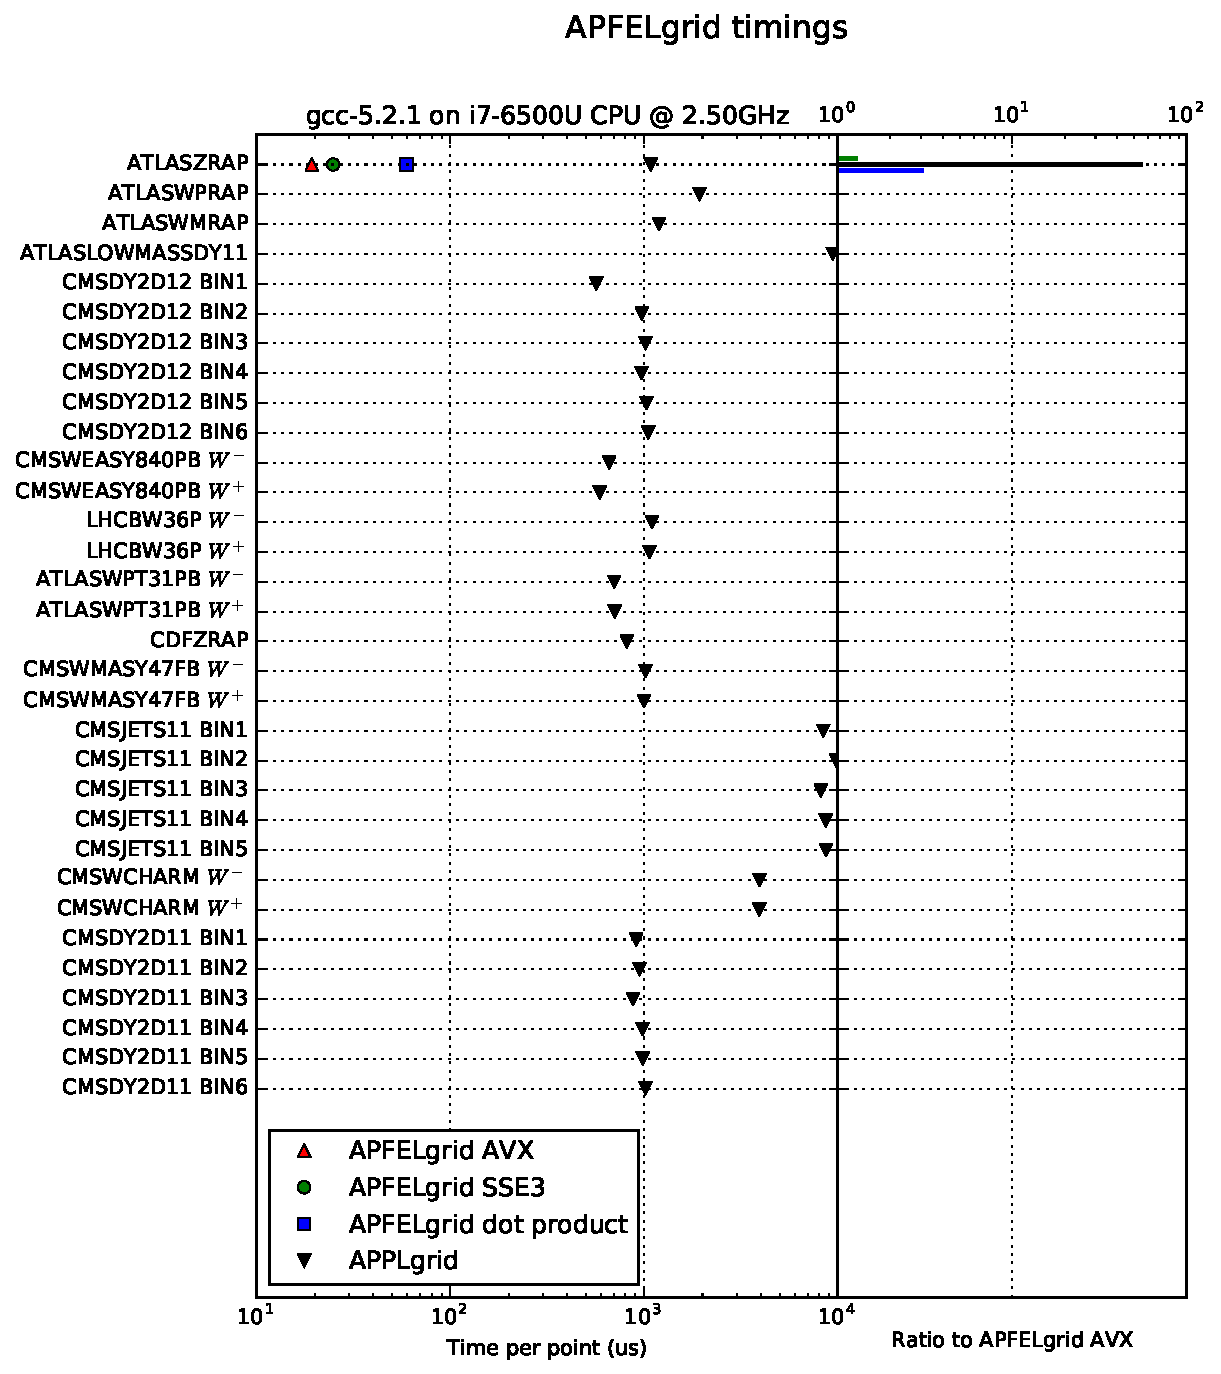
\includegraphics[scale=0.5]{plots/t0}
\caption{\small Performance comparisons between {\tt APFELgrid} with
  AVX, SSE3 and double precision convolution and {\tt APPLgrid}
  convolution time per point and process.}
\label{fig:benchmark}
\end{figure}
%%%%%%%%%%%%%%%%%%%%%%%%%%%%%%%%

%%%%%%%%%%%%%%%%%%%%%%%%%%%%%%%%%%%%%%%%%%%%%%%%%%%%%%%%%%
\begin{figure}[ph]
  \centering
  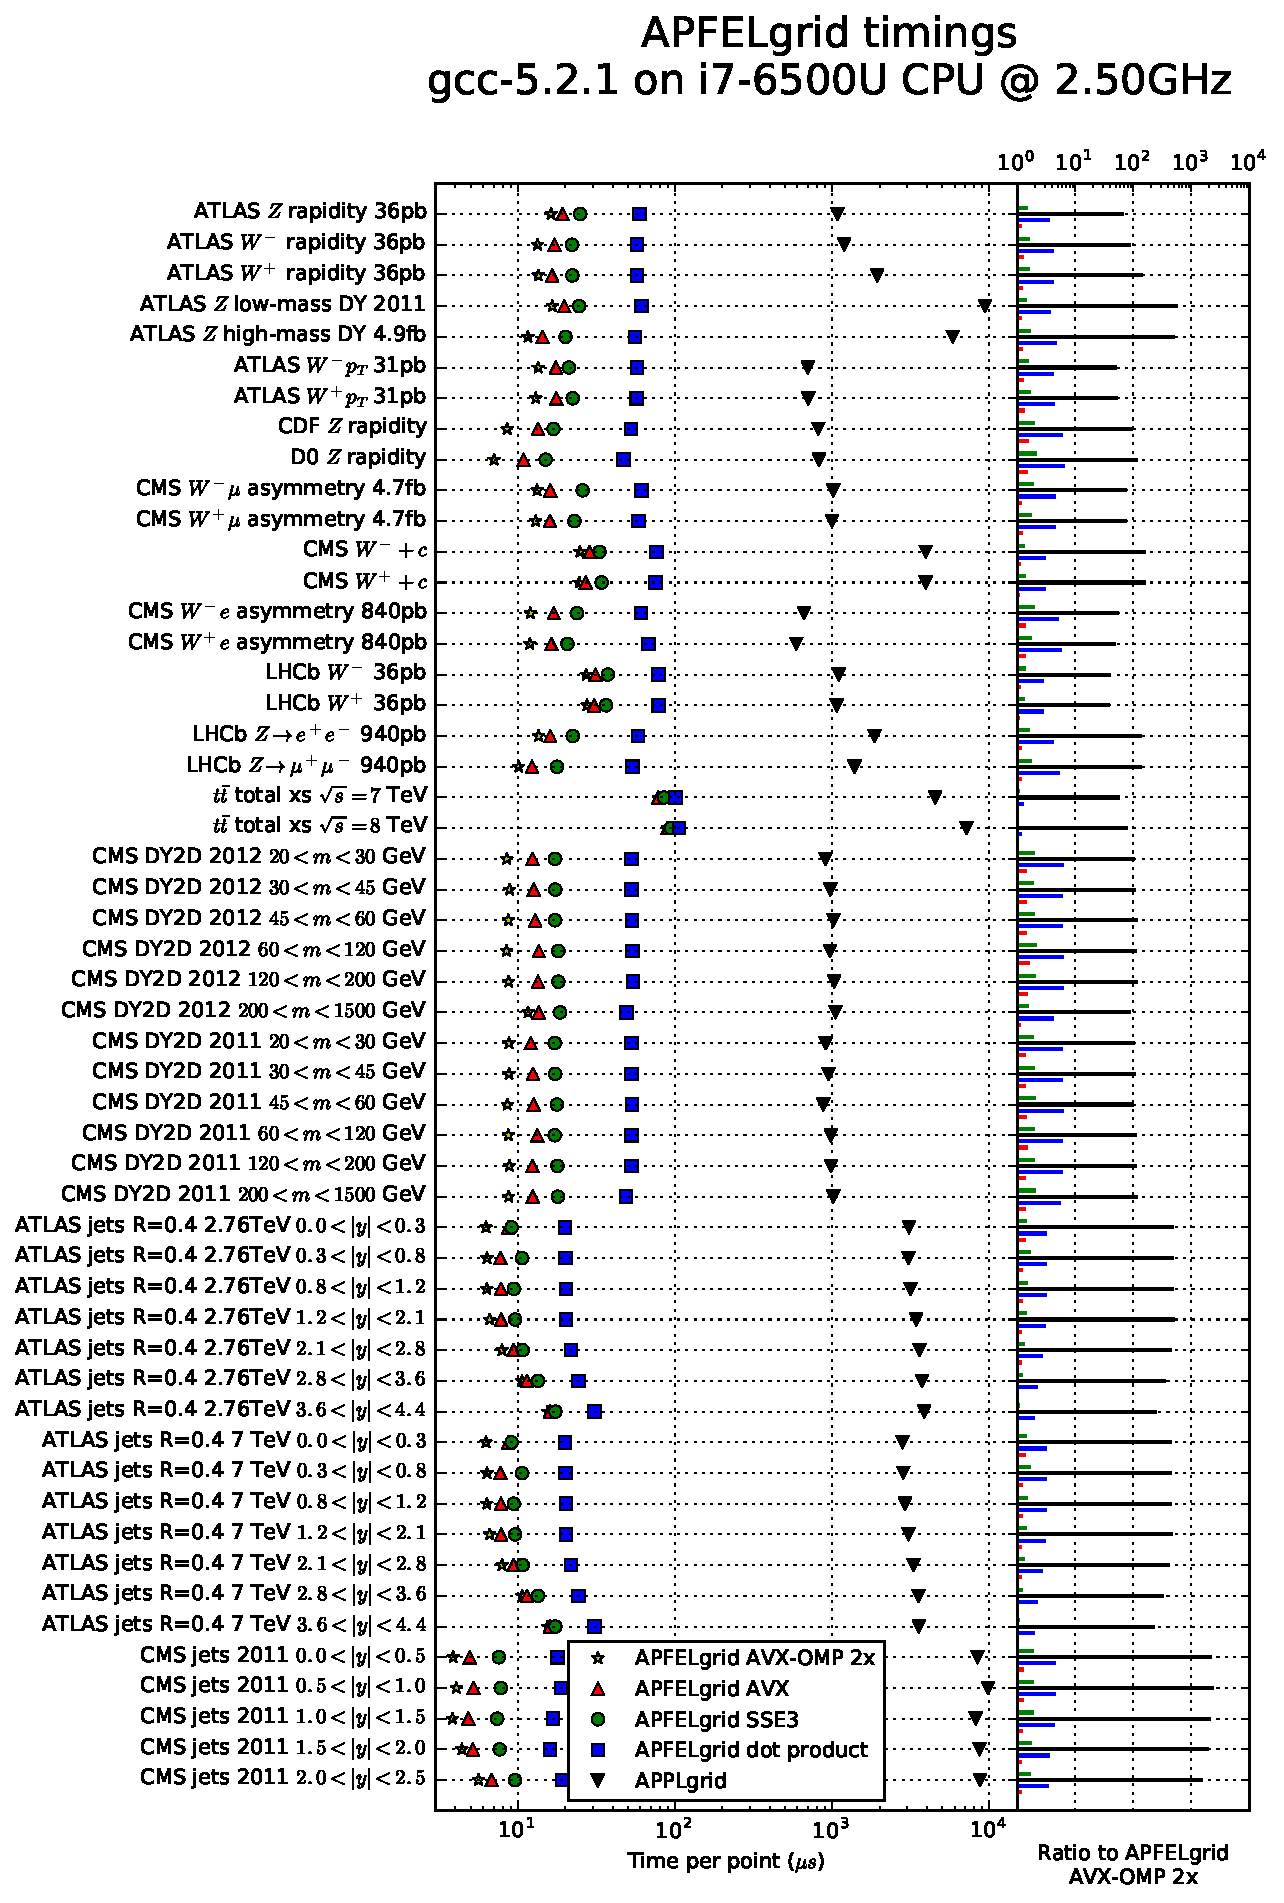
\includegraphics[scale=0.5]{plots/t0a}
\caption{\small Performance comparisons between {\tt APFELgrid} with
  AVX, SSE3 and double precision convolution and {\tt APPLgrid}
  convolution time per point and process.}
\label{fig:benchmark}
\end{figure}
%%%%%%%%%%%%%%%%%%%%%%%%%%%%%%%%

%%%%%%%%%%%%%%%%%%%%%%%%%%%%%%%%%%%%%%%%%%%%%%%%%%%%%%%%%%
\begin{figure}[ph]
  \centering                                      
  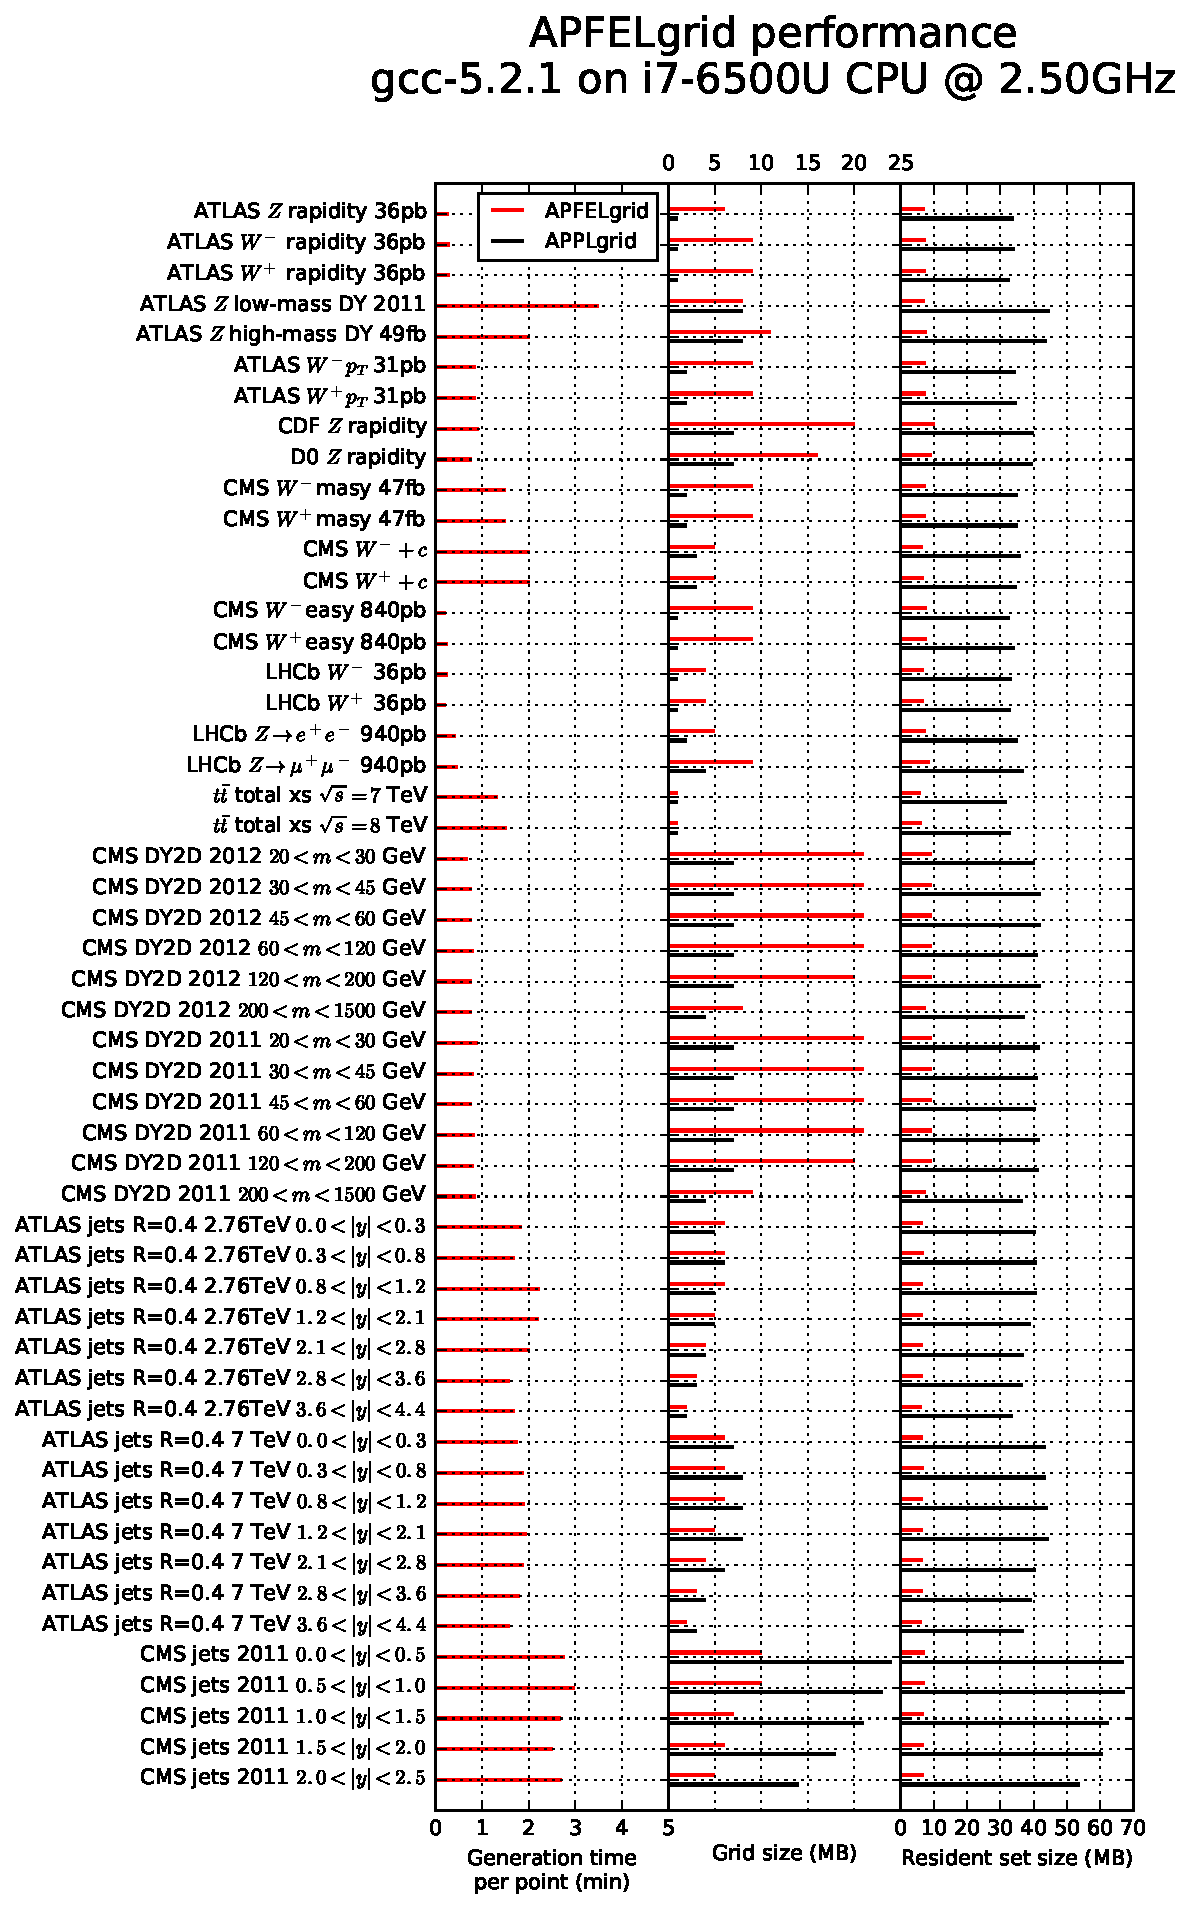
\includegraphics[scale=0.5]{plots/t0b}
\caption{\small Performance comparisons between {\tt APFELgrid} with
  AVX, SSE3 and double precision convolution and {\tt APPLgrid}
  convolution time per point and process.}
\label{fig:benchmark}
\end{figure}
%%%%%%%%%%%%%%%%%%%%%%%%%%%%%%%%



%% The Appendices part is started with the command \appendix;
%% appendix sections are then done as normal sections
%% \appendix

%% \section{}
%% \label{}

%% References
%%
%% Following citation commands can be used in the body text:
%% Usage of \cite is as follows:
%%   \cite{key}         ==>>  [#]
%%   \cite[chap. 2]{key} ==>> [#, chap. 2]
%%

%% References with bibTeX database:

\bibliographystyle{elsarticle-num}
\bibliography{paper.bib}

%% Authors are advised to submit their bibtex database files. They are
%% requested to list a bibtex style file in the manuscript if they do
%% not want to use elsarticle-num.bst.

%% References without bibTeX database:

% \begin{thebibliography}{00}

%% \bibitem must have the following form:
%%   \bibitem{key}...
%%

% \bibitem{}

% \end{thebibliography}

\end{document}

%%
%% End of file 
